The tape player is the central audio component of the module. 
It manages recording of incoming audio into a ping-pong buffer pair, and plays back the recorded content at a variable pitch determined by the V/oct CV input and the pitch slide potentiometer.

%TODO: visualization of Double Buffer in State machine

\paragraph{State Machines}

The tape player uses two independent FSMs (see below Figure \ref{fig:tape-player-fsms}): one for playback state (\texttt{play\_state\_t}: \texttt{STOPPED} / \texttt{PLAYING}) and one for 
recording state (\texttt{rec\_state\_t}: \texttt{IDLE} / \texttt{RECORDING} / 
\texttt{REREC} / \texttt{DONE}). 
Commands are delivered via a FreeRTOS queue 
(\texttt{tape\_cmd\_q}), decoupling the control interface from the audio processing 
path.

\begin{figure}[H]
	\centering
	\makebox[\textwidth][c]{%
		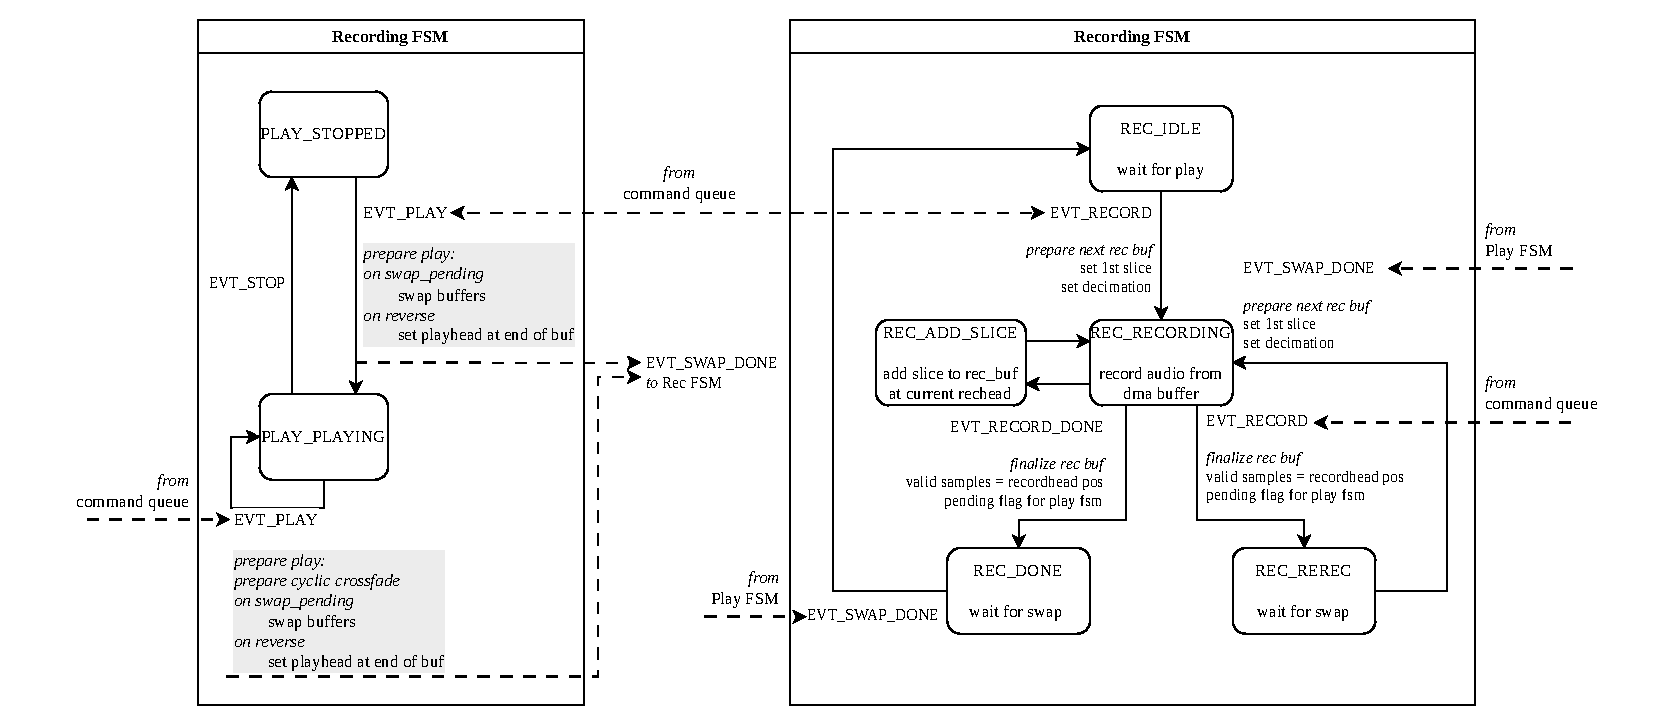
\includegraphics[width=1.15\textwidth]{../images/tape_player/tape_player_fsm.drawio.pdf}
	}
	\caption{Tape Player Component Record and Play FSMs}
	\label{fig:tape-player-fsms}
\end{figure}



\paragraph{Double Buffering and Buffer Structure}

Audio is stored in a \texttt{tape\_buffer\_t} struct, which holds two 16-bit sample buffers -- one per stereo channel -- along with metadata:

\begin{minted}{c}
typedef struct {
	int16_t* ch[2];          // ch[0]=L, ch[1]=R
	uint32_t size;           // samples per channel
	uint32_t valid_samples;  // valid recorded samples
	uint8_t  decimation;     // decimation factor
	uint32_t slice_positions[MAX_NUM_SLICES];
	uint32_t num_slices;
} tape_buffer_t;
\end{minted}

Two \texttt{tape\_buffer\_t} instances are maintained at all times — one for active playback and one for recording. 
When a new recording is complete, the buffers are swapped atomically, allowing uninterrupted playback during re-recording.

% TODO add in figure to show Double Buffer handling




\paragraph{Crossfade System}

Four \texttt{crossfade\_t} instances handle different transition scenarios: a retrigger crossfade (\texttt{xfade\_retrig}), a cyclic loop crossfade (\texttt{xfade\_cyclic}), and simple fade-in/fade-out envelopes at the start and end of playback. 

Each crossfade maintains its own secondary playhead position (\texttt{pos\_q48\_16}) and a fade accumulator (\texttt{fade\_acc\_q16}) that advances independently of the main playhead. 
This independence is important at low pitch factors: when the main playhead advances by only a fraction of a sample per output step, tying the fade curve to the playhead position would cause the crossfade to progress extremely slowly and produce audible stepping. 
By decoupling the fade accumulator from the playhead, the crossfade always completes in a fixed wall-clock time regardless of pitch.

The fade curve shape is a quarter period of a sine function, stored as a pre-computed lookup table (LUT). 
A raised cosine / quarter-sine fade produces a perceptually smooth gain transition — the slope starts at zero, rises through the midpoint, and flattens again at unity — avoiding the abrupt onset and offset that a linear ramp would produce at the boundaries. 
The fade accumulator (\texttt{fade\_acc\_q16}) is a Q16.16 fixed-point phase that indexes into the LUT, advancing by \texttt{step\_q16} each sample. 
The step size is calculated from the desired fade length and the LUT size, so the LUT is traversed exactly once over the duration of the crossfade:

\[
\texttt{step} = \frac{N_{\text{LUT}}}{\texttt{fade\_len}}
\]

For crossfades between two buffer regions (retrigger and cyclic), a second buffer pointer (\texttt{buf\_b\_ptr\_l}, \texttt{buf\_b\_ptr\_r}) tracks the outgoing audio segment, while the main playhead reads the incoming segment. 
The two signals are blended using complementary fade-in and fade-out curves derived from the same LUT, ensuring a constant-power crossfade.

\paragraph{Playback Trigger Modes}

Three distinct trigger scenarios are handled by the play FSM, each requiring a 
different crossfade strategy:

\begin{description}
	\item[Trigger from idle] The simplest case. The playhead is positioned at the 
	selected slice start and a fade-in is armed. No crossfade is needed since 
	there is no outgoing audio to blend with.
	
	\item[Retrigger --- same buffer] When a play event arrives while the same 
	buffer is already playing, the \texttt{xfade\_retrig} secondary playhead is 
	pointed directly at the current position in the playback buffer — no copy is 
	needed — and the main playhead jumps to the new slice start. The outgoing tail 
	fades out while the new start fades in, producing a click-free retrigger.
	
	\item[Retrigger --- new buffer pending] When a new recording is waiting to be 
	promoted (\texttt{swap\_bufs\_pending}), the outgoing tail samples are first 
	copied into a static temporary buffer (\texttt{xfade\_retrig\_temp\_buf}) 
	before the swap, since after the swap the old playback buffer becomes the 
	record buffer and its contents may be overwritten. The buffers are then 
	swapped, and the crossfade fades from the saved temporary buffer into the 
	beginning of the new playback buffer, ensuring a seamless transition across 
	the buffer switch.
\end{description}

In all retrigger cases, the available sample count between the current playhead 
and the end of valid data is checked before arming the crossfade. If fewer samples 
are available than the full crossfade length, \texttt{temp\_buf\_valid\_samples} is 
clamped accordingly to prevent out-of-bounds reads at the buffer and LUT 
boundaries.

\paragraph{Playhead and Pitch}

The playhead position is tracked as a Q48.16 fixed-point number (\texttt{pos\_q48\_16}): the upper 48 bits index into the sample buffer and the lower 16 bits carry the fractional offset used by the Hermite interpolator (Section~\ref{sec:numerical-architecture}). 
A separate \texttt{curr\_phase\_inc} and \texttt{target\_phase\_inc} allow smooth pitch transitions by slewing the increment toward the target value each block. 
The pitch interpolation system is examined in detail in Focus Point 1 
(Section~\ref{sec:focus-1-pitch-interpolation}).

\paragraph{Decimation}

A configurable decimation factor reduces the effective sample rate during recording and playback, extending the maximum recording time at the cost of audio bandwidth. 
The \texttt{grit} parameter is derived from the decimation factor and controls the blend between Hermite and ZOH interpolation, introducing intentional degradation as an aesthetic effect.
%TODO more detailed view into this?